
\documentclass{article}

\usepackage[utf8]{inputenc}
\usepackage{braket}
\usepackage{enumitem}
\usepackage{multirow}
\usepackage{xcolor}
\usepackage[T1]{fontenc}
% \usepackage[french]{babel}
\usepackage{amssymb}
\usepackage{mathtools}
\usepackage{ntheorem}
\usepackage{amsmath}
\usepackage{amssymb}
\usepackage[ a4paper, hmargin={2cm, 2cm}, vmargin={2cm, 2cm}]{geometry}
\usepackage{capt-of}

\usepackage{tikz}
\usetikzlibrary{angles,quotes}

\theoremstyle{plain}
\theorembodyfont{\normalfont}
\theoremseparator{~--}
\newtheorem*{define}{Definition}%[section]
\newtheorem*{ex}{Example}%[section]
\newtheorem*{obs}{Observation}%[section]

\newcommand{\norm}[1]{\left\lVert#1\right\rVert}

\usepackage{hyperref}
\hypersetup{
    colorlinks,
    citecolor=black,
    filecolor=black,
    linkcolor=blue,
    urlcolor=blue
}

\title{Lambda Calculus and category theory}
\author{Valeran MAYTIE}
\date{}

\begin{document}
  \maketitle

  \tableofcontents

  \section{Introduction}

  \paragraph{Boole} :
    \begin{itemize}
      \item
        If you consider propositions (no quantifiers) of
        \underline{classical logic} : $A ::= P | A \wedge B | \neg A | A \wedge B |
        \top | \bot $
      \item
        \underline{Ordered} by logical implication $A \leq B \Leftrightarrow A
        \Rightarrow B$, $A$ implies $B$ or $A \vdash B$
    \end{itemize}

    \underline{Observation} $A \wedge B \leq A, A \wedge B \leq B$. moreover if
    $C \leq A$ and $C \leq B$ then $C \leq A \wedge B$ (for all proprieties)

    Which means that $A \wedge B$ define a infimum of $A$ and $B$ (greatest lower
    bound, or \underline{glb})

  \define $A \Rightarrow B = (\neg A) \vee B = \neg (A \wedge \neg B)$.

  \hspace{5mm}

  Observation : \begin{itemize}
    \item $A \wedge (A \Rightarrow B) \leq B$
    \item $A \vee \neg A \leq \text{true}$
    \item $A \wedge \neg A \geq \text{false}$
  \end{itemize}\paragraph{Frege} Ideography (first proof system)

  The idea that a mathematical proof is a mathematical object. In particular
  there may be different proofs of a proposition $A$ formula.


  \begin{center}
  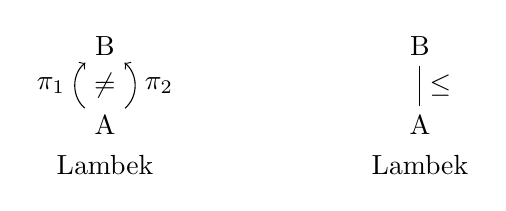
\begin{tikzpicture}
    \node (A) at (-2, 0) {A};
    \node (B) at (-2, 1) {B};
    \node at (-2, 0.5) {$\not =$};

    \draw[->] (A) to [bend right=50] node [right] {$\pi_2$} (B);
    \draw[->] (A) to [bend left=50]  node [left ] {$\pi_1$} (B);

    \node at (-2, -0.5) {Lambek};

    \node (A) at (2, 0) {A};
    \node (B) at (2, 1) {B};

    \draw (A) to node [right] {$\leq$} (B);
    \node at (2, -0.5) {Lambek};

  \end{tikzpicture}
  \end{center}


  Lambek understood connection between:

  \begin{center}
  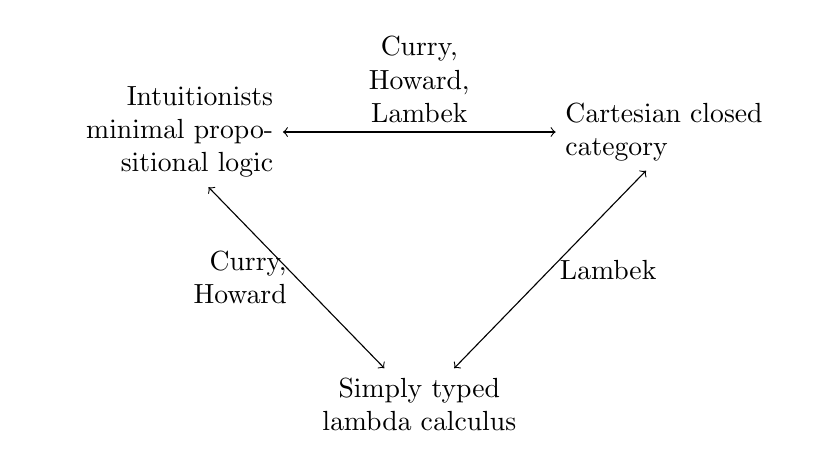
\begin{tikzpicture}
    \node[text width=3cm, anchor=west] (Cat) at (30:2) {Cartesian closed category};
    \node[text width=3cm, align=right, anchor=east] (Log) at (150:2) {Intuitionists minimal propositional logic};
    \node[text width=3cm, align=center, anchor=north] (Lam) at (270:2) {Simply typed lambda calculus};

    \draw [<->] (Cat) edge node[above, text width=2cm, align=center] {Curry, Howard, Lambek} (Log);
    \draw [<->] (Cat) edge node[right] {Lambek} (Lam);
    \draw [<->] (Log) edge node[left, text width=2cm, align=right] {Curry, Howard} (Lam);
  \end{tikzpicture}
  \end{center}

  \define A monoid $(M, \bullet, e)$ is a set $M$ equipped with a binary
  operation $\bullet : M \times M \to M$ with a neutral element $e \in M_e : M^0
  \to M$ satisfying two equations :

  \begin{itemize}
    \item (associativity) $\forall x, y, z \in M, x \bullet (y \bullet z) = (x
      \bullet y) \bullet z$
    \item (neutrality) $\forall x, \in M, x \bullet e = x = e \bullet x$
  \end{itemize}

  \ex $(\mathbb N, +, 0), (\mathbb Z, +, 0), (\mathbb N, \times, 1)$ and any
  group.

  Free monoid on a set (=alphabet) $A$. % todo: phrase qui veut rien dire ici
  $A^*$ contains finite sequences of element $A$ $w = [a_1 \ldots a_n]$

  \begin{itemize}
    \item Binary operation is concatenation.
    \item Neutral element is the empty word.
  \end{itemize}

  \section{Categories, functors, natural transformations}

  \define A category $\mathcal C$ is a \underline{graph}
    \begin{itemize}
      \item Whose nodes are called objects
      \item Whose edges are called morphism/maps/arrow.
    \end{itemize}

    The objects of $\mathcal C$ form a \underline{class} of objects.

    Every pair of object $A,B$ comes with a set $Hom(A, B)$ of morphisms
    $A \xrightarrow{f} B$, $f \in Hom(A, B)$

    The graph is equipped with:

    \begin{itemize}
      \item A morphism $id_A \in Hom(A, A)$ for all object $A$ of $\mathcal C$
      \item A composition defined as a function $\circ_{A,B,C}: Hom(B, C)
        \times Hom(A, B) \to Hom(A, C)$ for every objects $A,B,C$ of
        $\mathcal C$

        It satisfying the following equation :
        \begin{itemize}
          \item associativity :
            \begin{center}
            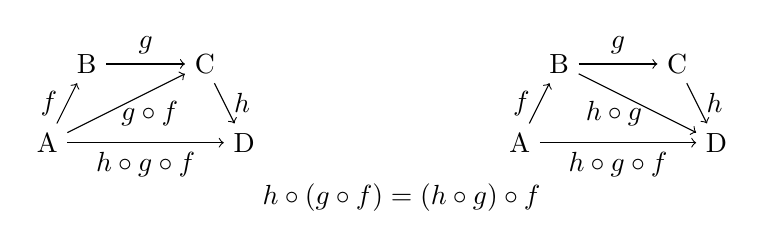
\begin{tikzpicture}
              \node (A) at (-4.5, 0) {A};
              \node (B) at (-4, 1) {B};
              \node (C) at (-2.5, 1) {C};
              \node (D) at (-2, 0) {D};

              \draw[->] (A) edge node[left] {$f$} (B) (B) edge node[above] {$g$} (C)
                        (C) to node[right]{$h$} (D);
              \draw[->] (A) to node[below] {$h \circ g \circ f$} (D);
              \draw[->] (A) to node[pos=0.7, below] {$g \circ f$} (C);

              \node (A) at (1.5, 0) {A};
              \node (B) at (2, 1) {B};
              \node (C) at (3.5, 1) {C};
              \node (D) at (4, 0) {D};

              \draw[->] (A) edge node[left] {$f$} (B) (B) edge node[above] {$g$} (C)
                        (C) to node[right]{$h$} (D);
              \draw[->] (A) to node[below] {$h \circ g \circ f$} (D);
              \draw[->] (B) to node[pos=0.3, below] {$h \circ g$} (D);

              \node at (0, -0.7) {$h \circ (g \circ f) = (h \circ g) \circ f$};
            \end{tikzpicture}
            \end{center}

          \item neutrality :

            \begin{center}
            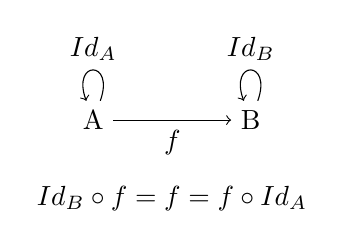
\begin{tikzpicture}
              \node (A) at (-1, 0) {A};
              \node (B) at (1, 0) {B};

              \draw[->] (A) to[out=70,in=110,looseness=8] node[above] {$Id_A$}(A);
              \draw[->] (B) to[out=70,in=110,looseness=8] node[above] {$Id_B$}(B);
              \draw[->] (A) to node[below] {$f$} (B);

              \node at (0, -1) {$Id_B \circ f = f = f \circ Id_A$};
            \end{tikzpicture}
            \end{center}
        \end{itemize}
    \end{itemize}

  \define A small category is a category whose class of object is a set.
  What we defined as a category is called ``\underline{locally small category}''.

  \ex

  \underline{Ordered Set}: Every ordered set $A$ defines a category.
    \begin{itemize}
      \item Objects: elements of $A$
      \item Morphisms : $a \to b \Leftrightarrow a \leq b$
        \[ Hom(a, b) =
          \begin{cases}
            \text{singleton} & a \leq b \\
            \emptyset
          \end{cases} \]

      The composition is defined by transitivity:

        \begin{center}
          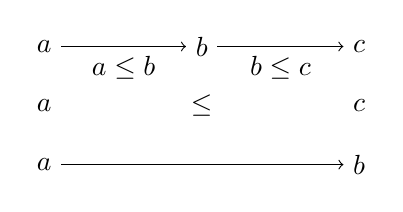
\begin{tikzpicture}
          \node (a) at (-2, 0) {$a$};
          \node (b) at ( 0, 0) {$b$};
          \node (c) at ( 2, 0) {$c$};

          \draw[->] (a) edge node[below] {$a\leq b$} (b)
                    (b) edge node[below] {$b\leq c$} (c);
          ;
          \node at (-2, -0.75) {$a$};
          \node at ( 0, -0.75) {$\leq$};
          \node at ( 2, -0.75) {$c$};
          \node (a) at (-2, -1.5) {$a$};
          \node (b) at ( 2, -1.5) {$b$};
          \draw[->] (a) edge (b);
        \end{tikzpicture}
        \end{center}
    \end{itemize}

    \define An ordered category $\mathcal C$ is a category where $Hom(A,B)$ is a
    singleton for all object $A, B $ of $\mathcal C$.

    \obs An ordered category is the same thing as a pre-order ($=$ trans, refl).

    \ex \underline{Monoid}
    \begin{itemize}
      \item A category with one object $*$, $M = Hom(*, *)$ define a monoid.
        \begin{itemize}
          \item $\circ : Hom(*, *) \times Hom(*,*) \to Hom(*, *)$
          \item $id_* \in M = Hom(*, *)$ define the neutral element
        \end{itemize}
      \item Conversely every monoid $M = (M, \bullet, e)$ defines a category
        $\mathcal B M$ or $\Sigma M$ with:
        \begin{itemize}
          \item One object $*$
          \item $Hom(*, *) = M$
          \item Composition defined by $y \circ x = y \bullet x$ with $e$, the neutral
        element.

        \end{itemize}

      \begin{center}
      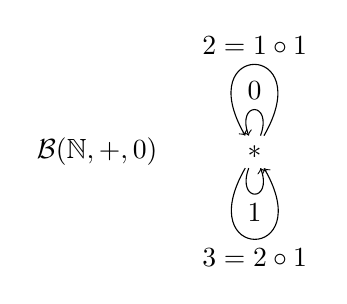
\begin{tikzpicture}
        \node at (-2, 0) {$\mathcal B (\mathbb N, +, 0)$};

        \node (*) at (0, 0) {$*$};

        \draw[->] (*) edge[out=70, in=110, looseness=8]  node[above] {0} (*);
        \draw[->] (*) edge[out=250,in=290, looseness=8]  node[below] {1} (*);
        \draw[->] (*) edge[out=60, in=120, looseness=15] node[above] {$2=1\circ 1$} (*);
        \draw[->] (*) edge[out=240,in=300, looseness=15] node[below] {$3=2\circ 1$} (*);
      \end{tikzpicture}
      \end{center}
    \end{itemize}
\end{document}
